%%% Thesis Introduction --------------------------------------------------
\chapter{Introduction}
\ifpdf
    \graphicspath{{Introduction/IntroductionFigs/PNG/}{Introduction/IntroductionFigs/PDF/}{Introduction/IntroductionFigs/}}
\else
    \graphicspath{{Introduction/IntroductionFigs/EPS/}{Introduction/IntroductionFigs/}}
\fi

%The Internet has had phenomenal success in the past 20 years, growing from a small research network to a global network that we use in a daily basis. The Internet is logically composed of end hosts interconnected by links and routers. When a host wants to communicate with other hosts, it uses the Internet Protocol (IP) to place information in packets, which are then sent to the nearest router. The router stores, then forwards, packets to the next hop, and through hop-by-hop routing, packets find their way to the desired destination. In other words, end hosts communicate through packet switching. With this communication technique, link bandwidth is shared among all information flows, and so these flows are statistically multiplexed on the link. The resulting service is best effort, in the sense that there are no deterministic guarantees.
%
%Optical burst switching (OBS) is a proposed new communications technology that seeks to expand the use of optical technology in switching systems. Optical technology has been used for a long time to carry information in fibers; however, the rapid growth of the Internet and the progress being made in Dense Wavelength Division Multiplexing (DWDM) creates an opportunity for more extensive use of optical resources in swithching and routing in the second generation of optical network systems. DWDM
%is a fiber-optic transmission technique. It is a multiplexing of many different wavelength signals onto a single fiber to obtain a set of parallel optical channels. Each channel uses a specific wavelength or color. This allows efficient fiber bandwidth and hence, limits the use of additional fibers. 
%
%\begin{figure}[!htbp]
%    \label{fig:trends}
%    \begin{center}
%        \leavevmode
%        \ifpdf
%        \resizebox{120mm}{!}{\includegraphics{pmf_thesis_img3}}
%        \else
%        \includegraphics[bb = 92 86 545 742, height=6in]{pmf_thesis_img3}
%        \fi
%        \caption[Trends of traffic demand]{Trends of traffic demand and the underlying technologies in the Internet [1998 = 100\%]. Trends for Silicon processing and router forwarding capacity are kept at the same value as today, despite talks of a slow down after 2004\cite{pablo03}}
%    \end{center}
%\end{figure}
%
%If the Internet is based on packet switching, why would I want to use optical burst switching? The answer is simple. There is a mismatch between the evolution rates of traffic and capacity of the Internet, but optical burst switching can help bridge the gap between demand and supply. recent advances in MEMS \cite{mems}, integrated waveguides \cite{waveguides}, optical gratings \cite{micromirrors}, tunable lasers, and holography have made possible very high capacity switch fabrics. And because of DWDM, single fibers have been able to
%transmit data at speeds up to 400Gb/s. Hence exchange rate will become the bottleneck of network rates \cite{bottleneck}. Optical burst switch network structure proposed in order to exploit the enormous bandwidth of DWDM technology, and overcome the bottleneck of the electron exchange rate.
%
%The novel idea of OBS networks is to keep the information in the optical domain as long as possible. This allows the system to overcome the limitations imposed by the electronic processing and opto-electronic conversion, leading to high speed data forwarding and high transparency. However, many challenging issues have to be solved in order to pave the way for an effective implementation of OBS. Contention, which may occur when two or more bursts compete for the same wavelength on
%the same link, is a critical issue. Many contention resolution methods have been proposed in the literature but many of them are very vulnerable to network load and may suffer severe loss in case of heavy traffic. So we need to develop a new congestion control scheme to prevent congestion collapse and keep OBS network throughput high.
%
\section{Methodology}
As mention above, the study intends to develop a new congestion control scheme for OBS. Thus, the following main question arise:

\begin{enumerate}

    \item How to indicate congestion state
    \item Design the feedback message packet
    \item How to determine edge router reaction
    \item How to measure the result 
    \item Does it work for any type of network application

\end{enumerate}

Each of the main questions was investigated by considering the following sub question:

\begin{table}[!htb]
    \label{tab:question}
    \centering
    \begin{tabular}{|c|l|}
        \hline
        No. & Questions \\
        \hline
        \multirow{2}{*}{1} & How to indicate congestion state \\\cline{2-2}
        & \hspace{5pt} What information should collect? \\
        & \hspace{5pt} Where can store this information? \\
        & \hspace{5pt} How to calculate the congestion threshold? \\
        & \hspace{5pt} The threshold can adjust dynamic?\\
        & \hspace{5pt} To finish this job, is it necessary to enhance core node? \\
        \hline
        \multirow{2}{*}{2} & Design the feedback message packet \\\cline{2-2}
        & \hspace{5pt} What field contain in the message packet? \\
        & \hspace{5pt} Is the size of message body minimum? \\
        & \hspace{5pt} When this congestion control message send to edge router?\\
        & \hspace{5pt} How often this message send to edge router?\\
        & \hspace{5pt} Which channel wiil be used to send this message?\\
        \hline

        \multirow{2}{*}{3} & How to determine edge router reaction \\\cline{2-2}
        & \hspace{5pt} Reduced delivery rate \\
        & \hspace{5pt} Select other idle path \\
        \hline

        \multirow{2}{*}{4} & How to measure result \\\cline{2-2}
        & \hspace{5pt} Assign various rank for different performance factor  \\
        & \hspace{5pt} Fairness to each factor \\
        & \hspace{5pt} Is effective when traffic load become higher \\
        & \hspace{5pt} Fairness to each edge router \\
        \hline

    \end{tabular}
    \caption{Questions and Sub-Questions}
\end{table}
\newpage
In this study, \verb|OPNET| and simulation will be utilized. Simulation is a cheap and quick method. It could also suggest analysis method. Nonetheless, it would a little hard to do a quantitative analysis. But it use to make a qualitative analysis to verify the simulation result.

\begin{figure}[!htb]
    \label{fig:methodology}
    \begin{center}
        \leavevmode
        \ifpdf
        \resizebox{120mm}{!}{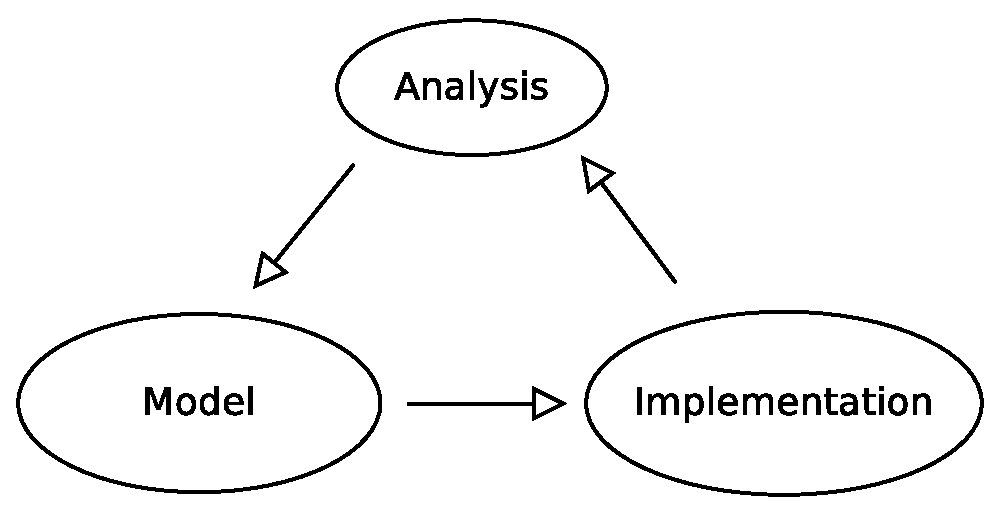
\includegraphics[height=6in]{methodology}}
        \else
        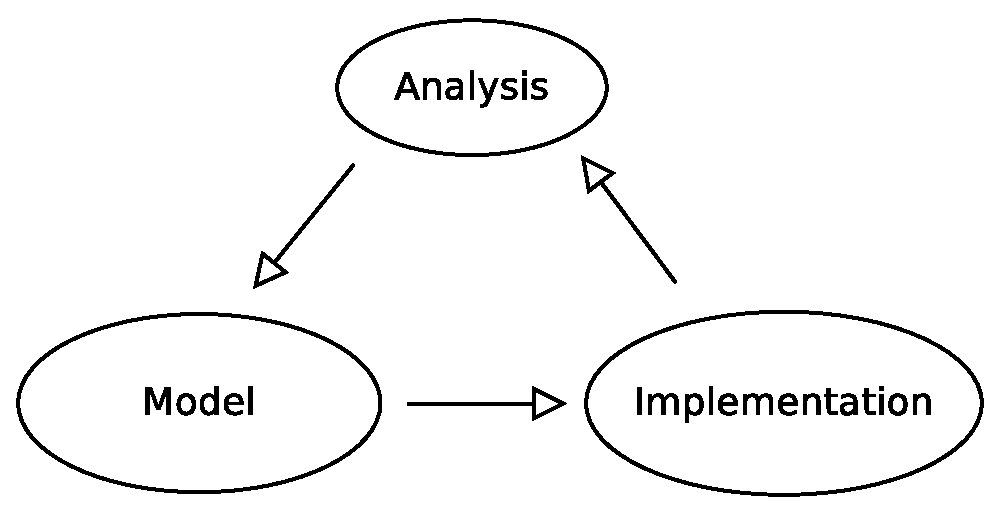
\includegraphics[bb = 92 86 545 742, height=6in]{methodology}
        \fi
        \caption{Instructional Simulate model for this study}
    \end{center}
\end{figure}

In the stage \verb|Model| and \verb|Implementation|, Use \verb|OPNET| as main tool. Because of \verb|OPNET| have provide a basic platform before progressing to the \verb|OBS| model. \verb|OPNET| simulation model library provide a series of simulation model for customer. On the basis of these simulation model, we can customize our network model and run a simulation. \verb|OPNET| simulation model library separate with the network simulation engine(\verb|OPNET|
Modeler,\verb|ITGuru|,Application DecisionGuru). This architecture is very convenient for model change and upgrade. For this study, we can deploy our congestion control algorithm to a \verb|OBS| network which build with \verb|OPNET| easily. 

To generate burst from all ingress node, we need to assume the arrive process follow certain distribution. That may be some common randomness processes. Such as negative exponential distribution, geometric distribution, drop-tail distribution. Thus we need to know how to generate this randomness process meet some distribution requirement. 

In order to measure our congestion control mechanism achievements. We need to setup a optimal target. In this study, that is maximum throughput and minimum burst loss and block ratio. It is hard to work out through pure analysis method. So we need to collect data from simulation. We can do some comparative experiments. Such as compare the throughput of two case. One with congestion control, the other without congestion control. Also, 
use some generally knowledge truth in queuing theory and probability theory to let us get closed optimal target step by step. It is a very good idea to make our data intuitive with data visualization technology.

\section{About congestion control}
To understand what is congestion control. The first question what causes congestion must be answer. Fortunately, the answer is simple, congestion occurs when the total traffic load is greater than network bottleneck capacity. Especially, OBS take one-way reservation to avoid the long end-to-end setup times and without buffer on intermediate router. Once contention occurs, some or all of data burst have to be dropped. Hence, contention is inherent to the OBS technique and
contention issue could affect tremendously the network performance in terms of burst blocked rate and throughput.

General speaking, the contention problem is due to the lack of communication between the nodes and the absence of global coordination between the edge routers and core routers. Congestion issue will lead to a large waste of resource due to drop of bursts on last one router before destination since fail to compete fail. Even worse, the network is statistical multiplexing, many burst may share a link, that lead to load is not balance over all core routers. Some core router may
overload, the others may be idle.  

There are two approaches to handle burst contention problem: bursts contention resolution and burst congestion control. The burst contention resolution approaches should have capacity to store burst with fiber delay lines (FDLs) \cite{fdl}, deflection routing \cite{deflection}, and wavelength conversion \cite{wavelenghtconv}. These approaches can reduce burst loss rate by absorbing short-term burst congestion. But if the burst congestion lasts long, all of above
approaches can't reduce burst loss rate anymore. Even worse, they may introduce longer end-to-end delay and enhance congestion impact. 

The burst congestion control mechanism handle the burst congestion by controlling the data burst transmission rate at the optical network edge. There are two paradigm to limit the source flow rate, refer as open-loop and closed-loop congestion control. The main different between these two mechanism is that closed-loop is dynamic adaptive system with feedback message. Open-loop is a per-define system without dynamic adjust stage.  There are two jointly operating mechanisms, namely a
burst congestion detection and a burst control algorithm in closed-loop network\cite{longterm}. Thus, in the feedback-based network it is required for the core router to work out 3W1H (what,where,when,how) question. What information should feedback to network edge router? Which router should monitor the network information and report to edge router? When this statistic result can detect the congestion and tell the edge router to reduce transmission
rate? On the other side the core router should tell when the edge router increase transmission rate to keep network throughput high? The last question is how to detect and predict the network congestion? How to guarantee fairness and self-organizing? 

%However, there are some misunderstandings about the causes and solutions of congestion control.
%
%\begin{enumerate}
%    \item Congestion is caused by the shortage of buffer space. The problem will be solved when the cost of memory becomes cheap enough to allow very large memory. Larger buffers are useful only for very short term congestions and will cause undesirable long delays. The long queue and long delay introduced by large memory is undesirable for many applications.
%
%    \item Congestion is caused by slow links. The problem will be solved when high-speed links become available. It is not always the case; sometimes increases in link bandwidth can aggravate the congestion problem because higher speed links may make the network more unbalanced. If two sources begin to send to destination 1 at their peak rate, congestion will occur at the switch. Higher speed links can make the congestion condition in the switch even worse.
%
%    \item Congestion is caused by slow processors. The problem will be solved when processor speed is improved. This statement can be explained to be wrong similarly to the second one. Faster processors will transmit more data per unit time. If several nodes begin to transmit to one destination simultaneously at their peak rate, the target will soon be overwhelmed. Congestion is a dynamic problem, and any static solutions are therefore not sufficient to solve the problem.
%        All the issues presented above: buffer shortage, slow link, slow processor are symptoms, not the causes of congestion. Proper congestion management mechanisms are more important than ever.
%\end{enumerate}

\cleardoublepage
\section{Motivation}

\begin{figure}[!htbp]
    \label{fig:ideal_congestion_control}
    \begin{center}
        \leavevmode
        \ifpdf
        \resizebox{90mm}{!}{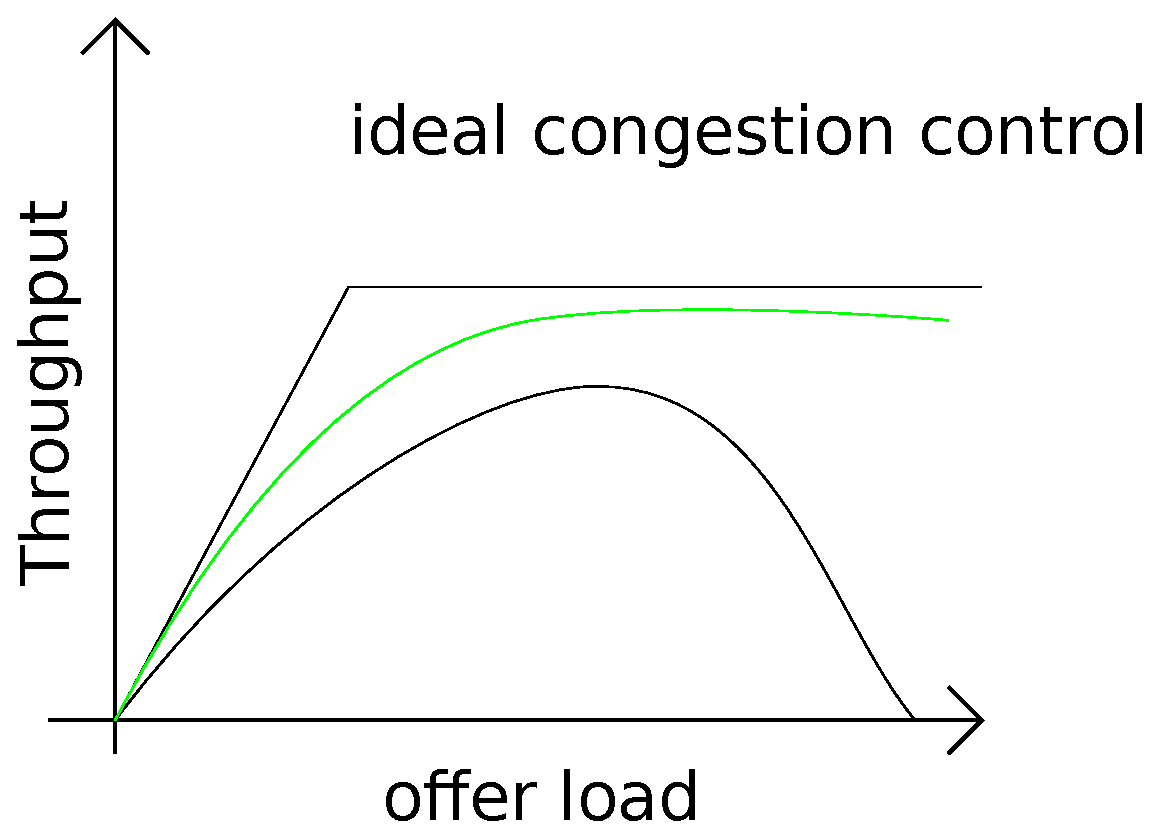
\includegraphics[height=6in]{ideal_congestion_control}}
        \else
        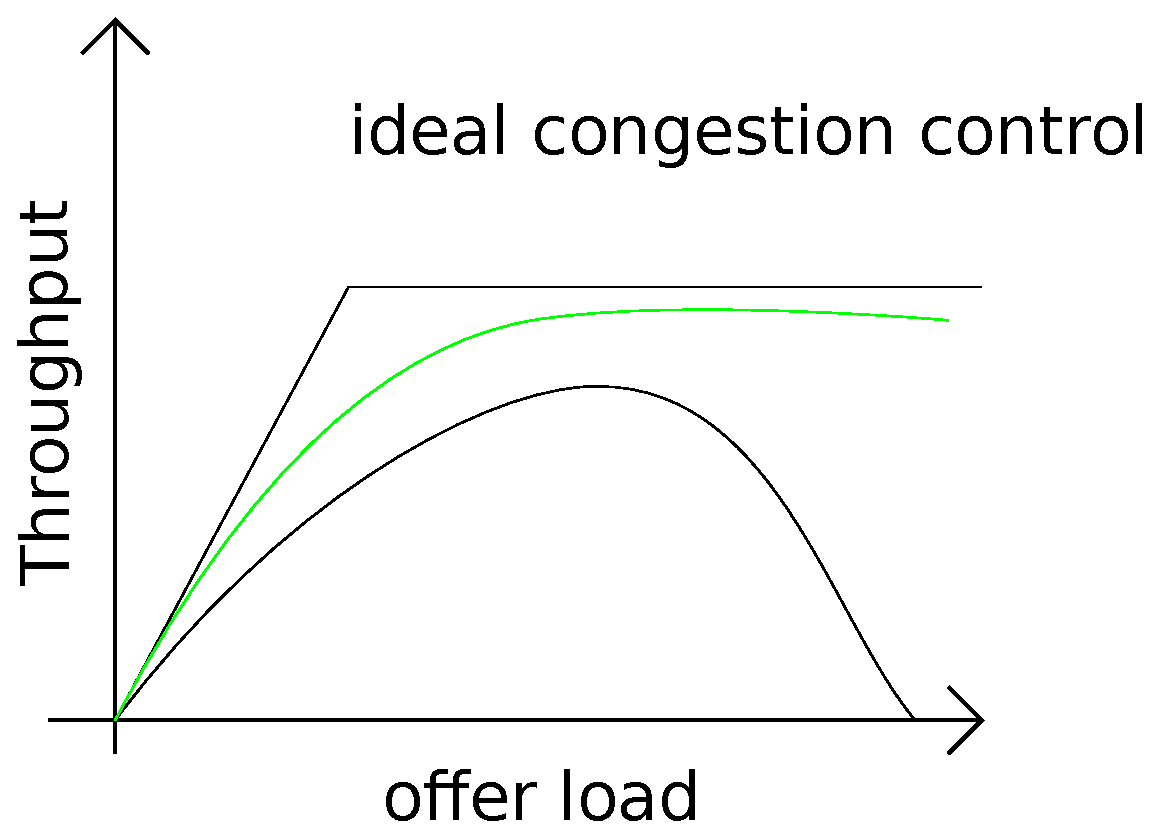
\includegraphics[bb = 92 86 545 742, height=6in]{ideal_congestion_control}
        \fi
        \caption{Congestion Control}
    \end{center}
\end{figure}

As figure \ref{fig:ideal_congestion_control} shows, The performance of network would reduce to zero if without any control. The ideal congestion control will enhance the network stability, and gain the capacity of network. However, in real network, the reaction delay much be token account. It only be closed to the ideal line. The green line show the real world congestion control. It may jitter since control packet loss or expired. In this study, I will develop a congestion control to
improve the throughput of network and reduce burst blocked probability.

There are several goals that congestion mechanism should achieve, the cost of implementation and deploy is cheap. That is said minimize additional hardware requirement and limited by router ability. Be fair among to all user.   

Congestion control is a comprehensive problem. The effective is very limited by control with any single method. Monitor and rate controller should co-operate to expand the effective. It may work with other mechanism, something like early drop packet, soft contention strategy.  

\section{Related Work}
As a new switching technology which has not been standardized yet, OBS faces many problems and challenges. However, there are also many researchers and new achievements. In resolving the issues of contention and the associated loss bursts issue. There are some other related studies. 

The most important and related study is contention resolution. As mention above, there are three ways to resolve burst contention. Fiber delay line, wavelength conversion and deflection routing by now. They are for a same goal. When contention occurs, they can buffer it instead of drop it. But these three method are not viable now. They all have their own shortcomings. Optical buffering currently can only be implemented using FDL. But this type of optical buffer is
usually small and it does not scale up. The wavelength may have some potential since the number of wavelengths that can be coupled together onto a single fiber continues to increase. In view of deflected routing, the end-to-end delay for an optical burst may be unacceptably high. But fortunately research on these contention resolution are going on. Once the breakthrough of these problems will also provide help for congestion control. 

Nowadays, IP packet switching already dominates global communications. But it cannot keep up with the Internet traffic demand. Many researchers are studying a new scheme to replace it. In electronic domain, ATM network has matured and is not far from being feasible. Other researcher have proposed integrate circuit switching in the core and packet switching in the edges as next generation network architecture. All of these efforts are aimed at accommodating for the traffic growth in the Internet. Study on the OBS can draw on
their achievements. Also include conventional TCP congestion control. 



%%% ----------------------------------------------------------------------


%%% Local Variables: 
%%% mode: latex
%%% TeX-master: "../thesis"
%%% End: 
